\section{WebRTC}

Рассмотрим WebRTC более подробно. WebRTC (Web Real-Time Communication -- коммуникация в режиме реального времени) -- это набор правил, позволяющий двум агентам вести двунаправленную безопасную коммуникацию в режиме реального времени.

\begin{figure}[ht]
\begin{center}
\scalebox{0.5}{
   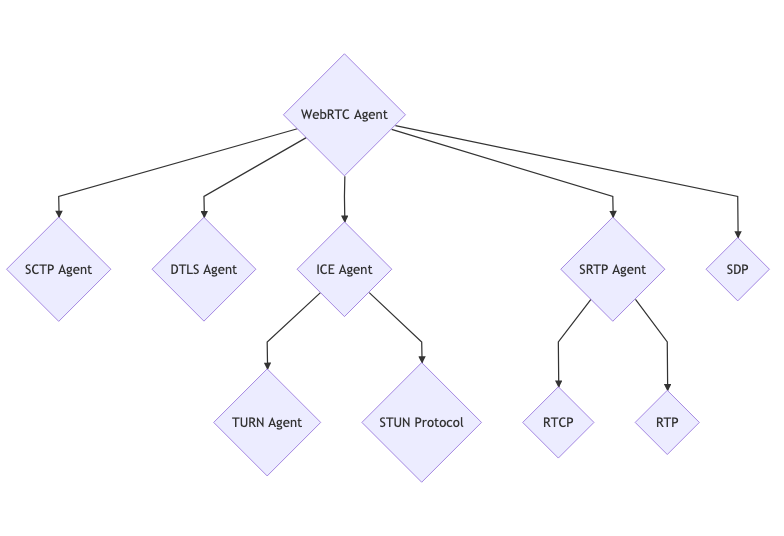
\includegraphics{images/webrtc_orchestr.png}
}

\caption{
\label{webrtc-orchestrator}
     WebRTC - оркестратор}
\end {center}
\end {figure}

Фактически WebRTC -- это оркестратор нескольких других протоколов, Рисунок ~\ref{webrtc-orchestrator}.

В процессе установки соединения можно выделить 4 основных этапа:
\begin{itemize}
	\item[--] Сигнализация;
	\item[--] Подключение;
        \item[--] Безопасность;
        \item[--] Коммуникация \cite{v3}.
\end{itemize}

Далее рассмотрим эти 4 этапа.

\subsection{Сигнализация}

Сигнализация -- это подготовка к совершению звонка. После обмена необходимой информацией участники могут общаться друг с другом напрямую.

Для совершения этого этапа WebRTC используется протокол SDP. Он позволяет двум участникам обменяться состоянием, необходимым для установки соединения. Протокол описания сессии определен в RFC 8866. Описание сессии представляет собой описание медиа (media description) и состоит из пар ключ/значение \cite{v21}.

\subsection{Подключение}

В WebRTC используется P2P (Peer-to-Peer) архитектура. Задача WebRTC обеспечить возможность двунаправленной коммуникации между двумя участниками.

ICE -- это протокол, который определяет наилучший способ для установки соединения между двумя участниками. Каждый участник определяет путь, по которому он может быть достигнут, затем ICE выбирает наиболее подходящую пару путей \cite{v22}.

\subsection{Безопасность}

Каждое соединения WebRTC аутентифицируется и шифруется. Таким образом, мы можем быть уверены, что третья сторона не видит того, что мы отправляем, и не может добавлять свои сообщения.

Для обеспечения безопасности соединения WebRTC использует DTLS и SRTP протоколы.

DTLS позволяет выполнить подготовку сессии и безопасно обмениваться данными между пирами. DTLS -- это клиент-серверный протокол, поэтому одна из сторон должна инициировать рукопожатие, в ходе него каждая из сторон генерирует сертификат. После завершения рукопожатия каждый сертификат сравнивается с его хешем, содержащим описание сессии, все это позволяет убедиться, что рукопожатие произошло с ожидаемым участником.

SRTP был разработан для безопасного обмена медиаданными. Для создания сессии SRTP мы инициализируем ее с помощью ключей, сгенерированных DTLS. После установки соединения стороны могут обмениваться зашифрованными медиаданными \cite{v23}.

\subsection{Коммуникация}

Для обмена данными WebRTC предоставляет каналы. Между двумя участниками может быть 65534 каналов. По умолчанию он гарантирует сохранение порядка сообщений.

Канал данных -- это абстракция потоков, из которых состоит SCTP. SCTP -- это транспортный протокол, являющийся альтернативой TCP и UDP, он определен в RFC 4960. Все настройки, связанные с продолжительностью существования канала и порядком доставки сообщений, передаются агенту SCTP \cite{v24}.

\pagebreak